% \begin{wrapfigure}{r}{0.4\textwidth}
%   % \begin{center}
%     \vspace{-25mm}
%     \includegraphics[scale=0.4]{img/.pdf}
%   % \end{center}
%   \caption{Approximation of static dependencies of an array summation program.\label{fig-sum}}
% \end{wrapfigure}

The paper presented a metalanguage for describing the semantics of a generic
instruction set architecture.
% The metalanguage closely resembles state
% transformers.
Multiple interpretations of the metalanguage terms allow us to evaluate the
semantics of instructions in different contexts without any modification of the
semantics itself. As the primary application, we present an approach to deriving
concurrency oracles of the instructions with only static data dependencies.

To handle instructions whose dependencies are dynamic, it is possible to use
conservative approximation of dependencies. For example, Fig.~\ref{fig-sum}
shows a dependency graph for a program  implementing the Euclidean algorithm
for computing the greats common divisor of two numbers that contains
a conditional branch instruction \hs{JumpZero} which modifies the instruction
counter \hs{IC} only if the previous instruction set the \hs{Zero} flag. In
this example we conservatively assume that \hs{JumpZero} always has a dependency
on \hs{IC}. Our future work includes applying the presented methodology to
extracting concurrency from real-world processor specifications, as described
in~\cite{mokhov2018formal}.

\vspace{-10mm}
\begin{figure}
\centerline{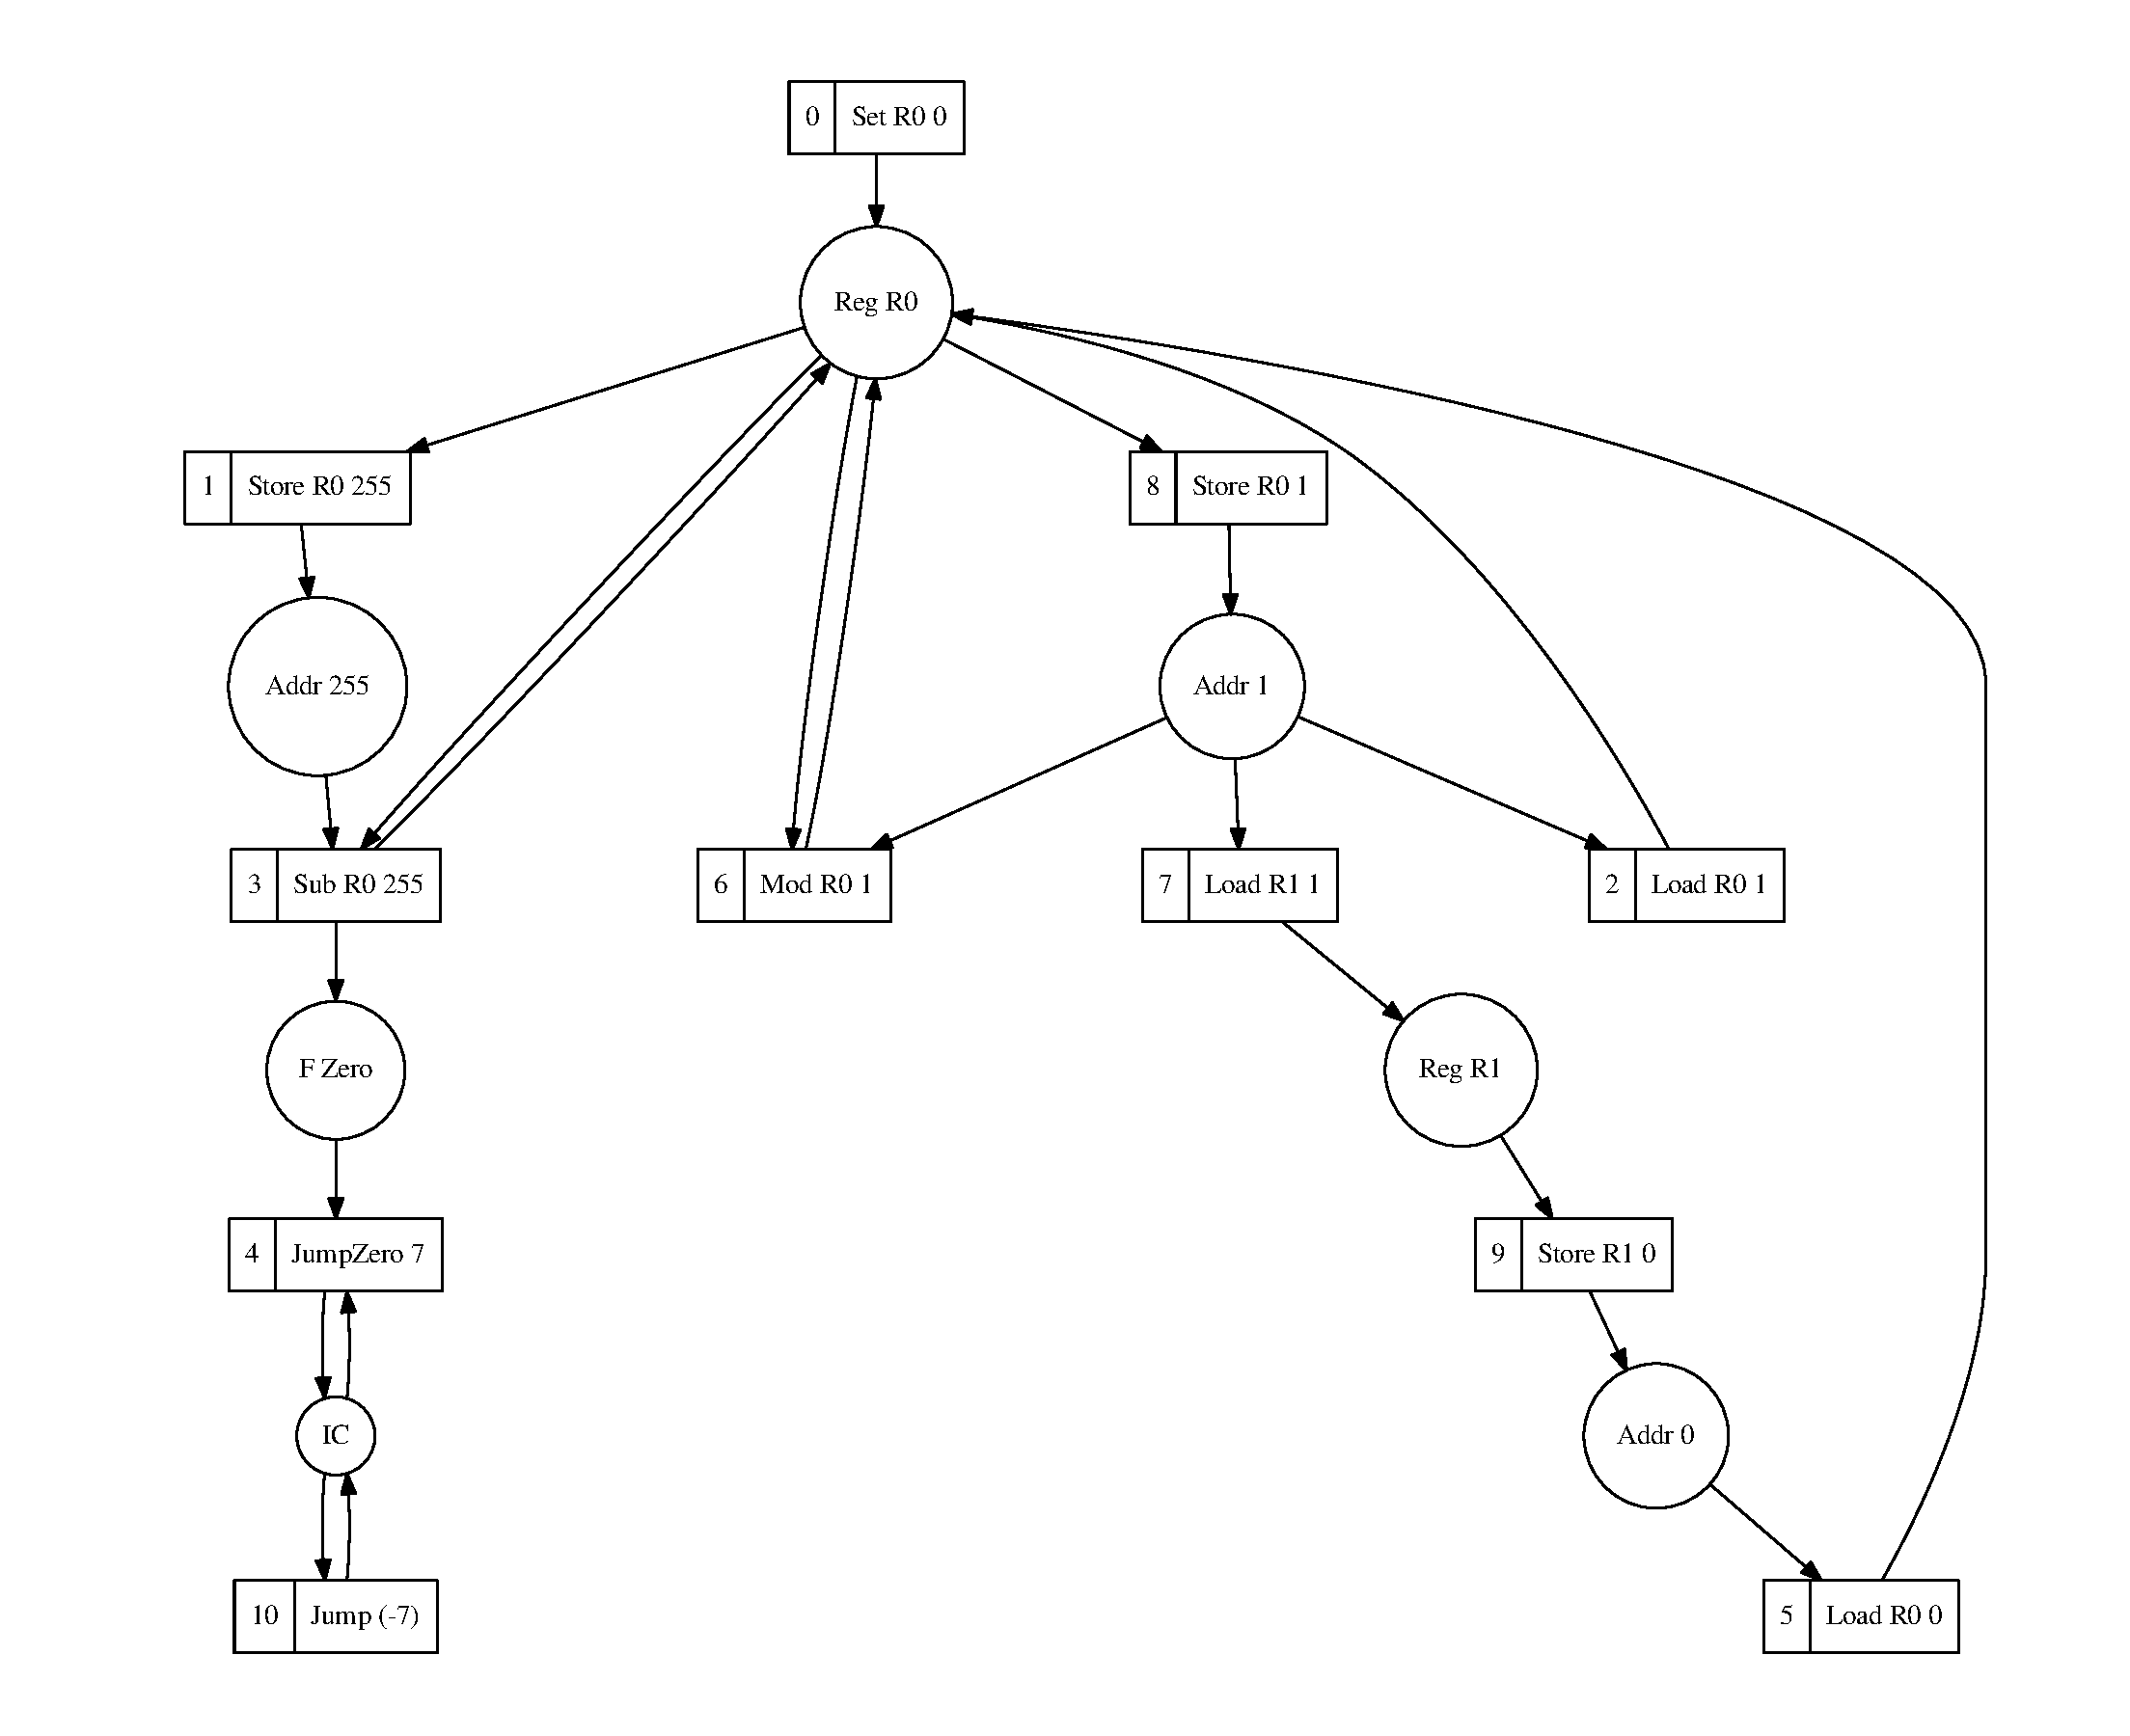
\includegraphics[scale=0.35]{img/gcd.pdf}}
\vspace{-7mm}
\caption{Approximation of static dependencies of an Euclidean algorithm implementation.\label{fig-sum}}
\vspace{-10mm}
\end{figure}
% \clearpage
